\documentclass[a4paper]{usiinfbachelorproject}

\captionsetup{labelfont={bf}}
%%%%%%%%%%%%%%%%%%%%%%%%%%%% PACKAGES %%%%%%%%%%%%%%%%%%%%%%%%%%%%%
\usepackage{float}
\usepackage{amsmath}
\usepackage{hyperref}
%%% Main Body %%%

\author{Daniel Dorigo }

\title{\textbf{PERNER - A Lightweight RoBERTa-Based, Task-Specific NER Model for Person Proper Noun Recognition}}
\subtitle{Subtitle}
\versiondate{\today}

\begin{committee}
%With more than 1 advisor an error is raised...: only 1 advisor   
\advisor[Universit\`a della Svizzera Italiana, Switzerland]{ }{prof. Monica }{Landoni }
%You can comment out  these lines if you don't have any assistant
%\coadvisor[Universit\`a della Svizzera Italiana, Switzerland]{ }{Firstname}{Lastname}

\end{committee}

\abstract {
This project presents the development of a specialized Named Entity Recognition (NER) \textbf{system} based on the RoBERTa-base architecture—a robustly optimized BERT pretraining approach—designed to accurately identify proper person names while distinguishing them from occupational titles in web-based textual content. The underlying model addresses critical limitations in general-purpose NER models that often misclassify job titles as person entities, especially in informal internet texts.

\\ \\ 
The proposed \textbf{model architecture} combines RoBERTa-generated contextual embeddings with a Conditional Random Field (CRF) layer for sequence labeling. It incorporates a composite loss function: focal loss to handle class imbalance and a custom boundary-weighted Dice loss to enhance entity span recognition. Additionally, a new \texttt{TITLE} label was introduced to explicitly distinguish occupational terms from actual person names, filling a gap in standard NER taxonomies.

\\ \\
Beyond the core model, the complete NER \textbf{system} implements additional components including a dynamic label configuration mechanism allowing flexible training with or without \texttt{TITLE} annotations, multiple architectural variants for differing computational budgets (simplified vs. full models), and confidence-based post-processing heuristics to enforce BIO sequence consistency. The system also features person-name substitution data augmentation and a two-phase hyperparameter optimization pipeline using Optuna: a coarse search with a lightweight model followed by a fine-tuning stage on the full architecture.

\\ \\
The final system demonstrated strong performance on the CONLL-2003 benchmark dataset while retaining a lightweight footprint appropriate for real-world deployment. These results show that task-specialized NER systems, built on lightweight yet expressive models, can aim to rival the accuracy of large-scale general-purpose approaches with significantly lower computational cost and energy requirements.

\\ \\
\textbf{Keywords}: Named Entity Recognition; Person Name Extraction; RoBERTa; Conditional Random Fields; Hyperparameter Optimization; Web Text Processing

}
\begin{document}
\maketitle
\tableofcontents
\newpage
%\listoffigures\newpage

\section{\textbf{Introduction}}
%Context.
Named Entity Recognition (NER) is a core task in Natural Language Processing (NLP), involving the detection and categorization of named entities-such as people, organizations, and locations-within unstructured text. With the widespread adoption of transformer-based models like BERT \cite{devlin-etal-2019-bert} and RoBERTa \cite{liu2019roberta}, the task has seen substantial improvements in accuracy across general benchmarks. However, applications requiring high precision in narrow domains, such as identifying proper nouns in informal or web-derived language, often expose the limitations of such broad models.
\\ \\
%Problem. 
This project was motivated by a real-world use case: extracting CEO names from company websites as part of a web-scraping pipeline. In this setting, existing NER systems frequently misidentified roles, titles, or nicknames as names, leading to unreliable outputs. These limitations highlighted the need for a specialized NER system with stronger performance in recognizing proper nouns-particularly under the noisy and non-standard conditions typical of internet text.
\\ \\
%Limitations in the State of the Art.
While general-purpose transformer models have raised the baseline for NER, they tend to conflate named entities with related but distinct concepts (e.g., job titles). Large Language Models (LLMs), such as GPT-3\cite{brown2020languagemodelsfewshotlearners} and GPT-4, have further broadened the approach by applying unsupervised, in-context learning across many NLP tasks. Yet, their generality often comes at the expense of consistency, interpretability, and efficiency-particularly in niche tasks where high recall and precision are critical. In such settings, even the most powerful LLMs may underperform due to their lack of domain-specific supervision \cite{DBLP:journals/corr/abs-2304-10428}.
\\ \\ 
%Contribution and Findings.
This work explores whether a fine-tuned, task-specific model based on the RoBERTa architecture can achieve competitive performance in recognizing proper nouns while maintaining computational efficiency. The core model incorporates several technical innovations: a hybrid RoBERTa-CRF architecture for improved sequence modeling, multi-component loss functions combining focal and Dice losses to address class imbalance and boundary detection, and a two-phase hyperparameter optimization strategy using Optuna for systematic parameter space exploration.

A novel TITLE label was introduced to disambiguate occupational titles from person names, improving output reliability in business and web contexts. The complete system features dynamic label configuration capabilities, allowing adaptation to datasets with or without title annotations. Additionally, a sophisticated data augmentation pipeline using person-name substitution and confidence-based post-processing heuristics enhance model robustness and prediction quality. The implementation supports both simplified and complex model variants, enabling deployment across different computational constraints while maintaining strong performance on standard benchmarks.




\section{\textbf{Background}}

To establish the theoretical and technical foundation for this specialized NER approach, this section examines the key technologies and methodologies that underpin the proposed system. The discussion begins with an analysis of current challenges in NER, particularly the difficulty of distinguishing proper nouns from related linguistic constructs. Subsequently, the fundamental architectures that enable modern NER systems—transformers and their derivatives—are reviewed to understand their capabilities and limitations. The section then explores the evolution from general-purpose to task-specific NER approaches, highlighting the trade-offs between broad applicability and specialized performance. Finally, the limitations of large language models in structured prediction tasks are examined, providing context for the focused approach adopted in this work.

\subsection{NER and the Challenge of Proper Noun Identification}

Named Entity Recognition (NER) has long been a core task in Natural Language Processing (NLP), aimed at identifying and classifying entities such as persons, locations, and organizations from raw text. While traditional models such as Conditional Random Fields (CRFs) laid the groundwork for early success, modern systems primarily rely on transformer-based architectures like BERT and RoBERTa, which leverage contextual embeddings to achieve state-of-the-art performance across a range of general-purpose benchmarks such as CONLL-2003 (a widely-used English NER dataset from the Conference on Natural Language Learning) and OntoNotes 5 (a large-scale multilingual dataset with comprehensive entity annotations)~\cite{inbook}.

Despite these advances, the broad focus of such models often results in overgeneralization when applied to more specialized or noisy domains. One recurring issue is the conflation of occupational roles (e.g., \textit{manager}, \textit{director}) with proper person names. This misclassification becomes particularly problematic in real-world applications such as web scraping, where distinguishing between a specific individual and their role is essential. For example, in a sentence like \textit{"The manager fired me,"} general-purpose models frequently tag \textit{manager} as a person entity, which may lead to semantic errors in downstream tasks such as automated document labeling, user profiling, or knowledge base population.

Treating proper nouns differently from common nouns, including occupational titles, is thus not merely a refinement but a practical necessity in domains like business intelligence, social media monitoring, and unstructured data mining. In the motivating use case for this project a web scraper aimed at extracting CEO names from company websites this distinction was foundational to accurate extraction.
\subsection{Transformers}
Transformers are a type of deep learning architecture introduced in the paper "Attention is All You Need" \cite{vaswani2023attentionneed}. Transformers use a mechanism known as self-attention to process entire sequences in parallel, in contrast to other models like Recurrent Neural Networks (RNNs) or Long-Short Term Memories (LSTMs), which process input sequences step by step. This enables the model to consider each word's relative importance in a sentence, regardless of its position. The primary goal is to effectively and adaptably capture the contextual relationships between words.

\subsection{BERT models:}
BERT (Bidirectional Encoder Representations from Transformers) is a deep learning model developed by Google\cite{devlin2019bertpretrainingdeepbidirectional} that has become a foundational architecture in modern natural language processing. BERT, which is based on the Transformer encoder, is intended to jointly condition on both left and right context in every layer in order to pre-train deep bidirectional representations. This implies that rather than only understanding words that come before or after, it can also understand the meaning of a word in relation to all of its surrounding words. Two unsupervised tasks are used to pre-train BERT on a large corpus of unlabeled text: Next Sentence Prediction (NSP), which teaches the model the relationship between paired sentences, and Masked Language Modeling (MLM), which masked random words in a sentence and taught the model to predict them. After pre-training, BERT can be fine-tuned with additional layers to perform specific NLP tasks such as question answering, text classification, or named entity recognition with minimal architecture changes.

\subsection{General-Purpose vs Task-Specific NER}

Although general-purpose NER models demonstrate impressive overall performance, they are not explicitly trained to handle fine-grained distinctions such as the separation of proper nouns from occupational roles. Evaluation benchmarks like CONLL-2003 include person entities as a broad category, but no widely adopted dataset exists for the narrower task of proper name extraction alone.

Furthermore, to the best of my knowledge, no prior work has introduced a dedicated label class to explicitly identify occupational titles. This omission reflects the underlying assumption of most NER pipelines: that entities can be categorized into a handful of coarse-grained types, without accounting for intra-category subtleties that may be critical in applied scenarios.

One study evaluating NER performance in a niche context philosophical texts\cite{weijers2025evaluation} found that even in constrained domains, specialized tuning and model choices matter. In that case, a trained version of Flair~\cite{akbik-etal-2019-flair} achieved the best F1 score (0.91), outperforming other models that used different methods (rule-based, LLMs with general-tuning...) on targeted tasks. This suggests that for subdomains of NER, specialization can rival or even exceed brute-force generalization.

\subsection{Large Language Models and the Limits of Generalization}

The recent emergence of large language models (LLMs) such as GPT-3 and GPT-4 has shifted attention toward unsupervised, in-context learning approaches for a variety of NLP tasks, including NER. In this paradigm, models generate responses based on prompt structure and context, often without requiring fine-tuning or labeled datasets. While this flexibility is appealing, it introduces significant drawbacks: hallucination, interpretability issues, and inconsistent behavior in low-resource or highly specific contexts.

As highlighted in GPT-NER by \cite{DBLP:journals/corr/abs-2304-10428}, LLMs are prone to various issues due to the intrinsic gap between the two tasks of NER and LLMs, NER is a sequence labeling task, while e LLMs are formalized under a text generation task.



\subsection{Positioning of This Work}

To address these limitations, this project focuses on a compact, task-specific NER fine-tuning system designed explicitly to identify proper person names while distinguishing them from occupational titles. In contrast to most prior work, which operates on broad entity categories, this approach narrows the scope of recognition to maximize precision and relevance in web-based content such as company pages, social media, and newsletters.

This work primarily builds upon established benchmarks such as CONLL-2003 and domain specific corpora that collect data from social media, while the system architecture is designed to handle informal and domain-specific linguistic patterns often absent in traditional training corpora.

In addition, a novel \texttt{TITLE} label was introduced to annotate occupational roles explicitly something not found in any of the surveyed literature. This provides the underlying model with an additional degree of supervision, allowing it to learn not just what a person name is, but also what it is not.

While hyperparameter optimization is a standard technique in machine learning, its application here via Optuna ensures that the model remains both lightweight and performant, without sacrificing adaptability to noisy input domains.

\section{\textbf{Technical Implementation}}

\subsection{System Architecture Overview}

The implemented NER system employs a modular architecture built around the HuggingFace Transformers ecosystem, featuring dynamic configuration management and flexible model variants. The core system supports two primary model architectures: a simplified RoBERTa-CRF model optimized for efficiency and a complex variant with enhanced attention mechanisms and multi-component loss functions.

\subsection{Dynamic Label Configuration System}

A key feature in this implementation is the dynamic label configuration system that automatically detects and adapts to different labeling schemes. The system implements a \texttt{get\_label\_config()} function that determines whether to include TITLE tags based on dataset characteristics or explicit configuration. This enables training on datasets with varying annotation schemas:

\begin{itemize}
    \item \textbf{Standard NER Schema}: Uses conventional B-PERSON, I-PERSON, and O labels for traditional person entity recognition.
    \item \textbf{Enhanced Schema with Titles}: Extends the label set with B-TITLE and I-TITLE tags to explicitly model occupational roles and honorifics.
\end{itemize}

Both schemas follow the BIO (Begin-Inside-Outside) tagging convention, where B- tags mark the beginning of an entity, I- tags mark tokens inside an entity (continuation), and O tags mark tokens outside any entity. This encoding ensures unambiguous entity boundary detection and supports multi-token entities.

The label configuration system maintains consistency across training, evaluation, and inference phases, automatically saving and loading configuration metadata to ensure reproducibility across experimental runs.

\subsection{Hybrid Model Architectures}

\subsubsection{Simplified RoBERTa-CRF Model}

The simplified variant (\texttt{SimplifiedRobertaCRFForTokenClassification}) combines RoBERTa's contextual embeddings with CRF sequential constraints for improved boundary detection. This architecture prioritizes computational efficiency while maintaining strong performance, making it particularly well-suited for hyperparameter exploration and optimization trials where rapid experimentation is essential:

\begin{itemize}
    \item Pre-trained RoBERTa-base backbone for contextual token representations
    \item Linear classification layer projecting hidden states to label space
    \item CRF layer enforcing valid BIO tag transitions
    \item Streamlined forward pass optimized for inference speed and rapid hyperparameter search
\end{itemize}

\subsubsection{Enhanced Complex Model}

The complex variant (\texttt{RobertaCRFForTokenClassification}) incorporates additional architectural components for improved performance on challenging datasets:

\begin{itemize}
    \item \textbf{Cross-Attention Span Classifier}: Implements multi-head attention mechanisms (parallel attention computations that allow the model to focus on different types of relationships simultaneously) to capture long-range dependencies within entity spans\cite{Tan_Qiu_Chen_Wang_Huang_2020}.
    \item \textbf{Relative Position Embeddings}: Enhanced attention computation with relative positional encodings for better entity boundary detection.
    \item \textbf{Parameterized Architecture}: Configurable attention heads, relative position windows, and dropout rates for fine-grained optimization.
\end{itemize}

\subsection{Multi-Component Loss Function Design}

The system implements a loss combination strategy addressing multiple aspects of NER performance:

\subsubsection{Focal Loss for Class Imbalance}

Focal loss is a specialized loss function designed to address class imbalance problems in classification tasks\cite{9624339}. Unlike standard cross-entropy loss, focal loss reduces the loss contribution from easily classified examples and focuses learning on hard, misclassified examples. This is particularly important in NER where non-entity tokens (O tags) vastly outnumber entity tokens, creating a severe class imbalance that can bias models toward predicting non-entities.

Implemented focal loss with parameterized class weights to address the inherent imbalance in NER datasets where entity tokens are significantly outnumbered by non-entity tokens:

\begin{equation}
    FL(p_t) = -\alpha_t(1-p_t)^\gamma \log(p_t)
\end{equation}

where $p_t$ is the predicted probability for the true class, $\alpha_t$ is a class-specific weighting factor that addresses class imbalance, and $\gamma$ is the focusing parameter that controls how much the loss focuses on hard examples. When $\gamma = 0$, focal loss reduces to standard cross-entropy loss; higher $\gamma$ values increasingly down-weight easy examples.

The implementation includes specific weighting for PERSON entities (\texttt{person\_weight}) and optional TITLE entity weighting when available in the label schema.

\subsubsection{Enhanced Boundary Dice Loss}

Dice loss measures the overlap between predicted and true entity spans.\cite{Li2019DiceLF} Unlike token-level losses that treat each position independently, Dice loss considers the entire entity span as a unit, making it particularly suitable for sequence labelling tasks where entity boundaries are crucial.

A boundary-weighted Dice loss implementation that emphasizes critical positions in entity spans:

\begin{itemize}
    \item \textbf{B-weight}: Enhanced importance for entity beginning tokens
    \item \textbf{I-end weight}: Focus on entity ending positions
    \item \textbf{Context weight}: Attention to pre-entity context tokens
\end{itemize}

This approach addresses common boundary detection errors that plague sequence labeling tasks.

\subsubsection{CRF Loss Integration}

Conditional Random Fields (CRF) are probabilistic models that consider the sequence structure in labeling tasks. Unlike independent token classification, CRFs model the dependencies between adjacent labels, ensuring that label transitions follow valid patterns.

The CRF component provides structured prediction capabilities, ensuring valid tag transitions and improving sequence-level consistency. The CRF weight parameter allows balancing between token-level and sequence-level optimization objectives \cite{PATIL20201181}.

\subsection{Advanced Training Features}

\subsubsection{Person-Name Substitution Augmentation}

Data augmentation in NER traditionally involves techniques like synonym replacement or sentence paraphrasing, but these can disrupt entity boundaries or change semantic meaning. Person-name substitution is a domain-specific augmentation technique that systematically replaces existing person names in the training data with alternative names from a curated dictionary, while preserving the original sentence structure and maintaining exact BIO tag alignment.

The data augmentation pipeline implements intelligent person name substitution that maintains semantic coherence while increasing name diversity:

\begin{itemize}
    \item Automatic extraction of person names from training corpora
    \item Integration with external name dictionaries for broader coverage
    \item Context-preserving substitution maintaining BIO tag consistency
    \item Configurable augmentation factors for controlled dataset expansion
\end{itemize}

\subsubsection{Confidence-Based Post-Processing}

A comprehensive post-processing system applies confidence-based heuristics to improve prediction quality:

\begin{itemize}
    \item Gap filling between high-confidence entity tokens
    \item Invalid transition correction (e.g., O → I-PERSON becomes O → B-PERSON)
    \item Noise suppression for isolated low-confidence predictions
    \item Configurable confidence thresholds optimized during hyperparameter search
\end{itemize}

\subsection{Two-Phase Optimization Pipeline}

The hyperparameter optimization system implements a sophisticated two-phase strategy using Optuna, an automatic hyperparameter optimization framework that employs advanced sampling algorithms like Tree-structured Parzen Estimator (TPE), a Bayesian optimization method that models the probability distribution of hyperparameters leading to good performance, to efficiently explore parameter spaces. Optuna's pruning capabilities allow early termination of unpromising trials, significantly reducing computational overhead during optimization.

The simplified model architecture is specifically employed throughout this optimization process to enable efficient parameter exploration while maintaining representative performance characteristics.

\subsubsection{Phase 1: Broad Exploration}
\begin{itemize}
    \item Wide parameter ranges covering architectural and training hyperparameters
    \item Median pruning for early termination of unpromising trials (a technique that stops training trials whose intermediate results fall below the median performance of completed trials)
    \item Reduced epoch count for faster iteration using the simplified model
    \item Parameter importance analysis for search space refinement
\end{itemize}

\subsubsection{Phase 2: Focused Refinement}
\begin{itemize}
    \item Concentrated search around promising parameter regions identified in Phase 1
    \item Statistical analysis of top-performing trials to define focused ranges
    \item Increased training epochs for more reliable performance estimates
    \item Enhanced pruning strategies for efficient resource utilization
\end{itemize}

The optimization pipeline automatically analyzes Phase 1 results, generates focused parameter ranges, and seamlessly transitions to Phase 2 search without manual intervention.

\vspace{1em}
\noindent
In summary, this work contributes a specialized, efficient alternative to general-purpose NER systems by:
\begin{itemize}
  \item Defining a narrow task proper name recognition that reflects specific real-world needs.
  \item Introducing a novel entity class for occupational roles, absent from prior NER taxonomies.
  \item Developing a robust system architecture capable of handling diverse text types and domains.
  \item Demonstrating that lightweight, supervised models can mitigate common failure cases in general-purpose and LLM-based systems.
\end{itemize}

   \subsection{Alternative Approaches Considered}

\subsubsection{Initial Weighted Trainer Approach}
Initially, an alternative training strategy was explored that leveraged a weighted trainer to address class imbalance by assigning different weights to samples during training. This approach aimed to emphasize less frequent entity classes such as B-PERSON and I-PERSON through token-level weighting.

However, significant limitations were observed:
\begin{itemize}
    \item \textbf{Sequential Training Bias}: When training on multiple datasets sequentially, the model developed strong bias toward the most recently seen dataset, causing performance degradation on earlier datasets
    \item \textbf{Token-Level Focus}: The approach prioritized individual token classification rather than holistic entity-level recognition
\end{itemize}

This approach was ultimately abandoned in favor of the current system, which addresses class imbalance through sophisticated multi-component loss functions and data augmentation strategies that proved more effective for balanced learning and entity segmentation.

\section{Approach}

\subsection{Training Procedure and Implementation Details}

Post-processing heuristics are used to correct common prediction errors. These rules operate on the model’s confidence scores and tag sequences:

\begin{itemize}
    \item Low-confidence "O" between entity tags may be converted to "I-PERSON".
    \item "I-PERSON" following "O" may be reclassified as "B-PERSON".
    \item Single-token "I-PERSON" spans are corrected to "B-PERSON".
\end{itemize}

This step improves boundary alignment and reduces entity fragmentation.

The training pipeline implements a sophisticated multi-stage approach that balances efficiency with performance optimization. The system supports both simplified and complex model variants, with automatic configuration based on experimental requirements.

\subsubsection{Model Initialization and Configuration}

The training system employs a dynamic configuration management approach that automatically adapts to different dataset schemas and experimental settings:

\begin{itemize}
    \item \textbf{Automatic Schema Detection}: The system automatically detects whether the dataset includes TITLE labels using the \texttt{detect\_label\_schema()} function
    \item \textbf{Dynamic Label Configuration}: The \texttt{get\_label\_config()} function generates appropriate label mappings, supporting both 3-label (O, B-PERSON, I-PERSON) and 5-label (O, B-PERSON, I-PERSON, B-TITLE, I-TITLE) schemes
    \item \textbf{Model Variant Selection}: Based on the \texttt{use\_simplified\_model} flag, the system initializes either the streamlined \texttt{SimplifiedRobertaCRFForTokenClassification} (optimized for rapid hyperparameter exploration) or the complex \texttt{RobertaCRFForTokenClassification} architecture (used for final training and deployment)
\end{itemize}

\subsubsection{Data Augmentation Pipeline}

The training process incorporates intelligent data augmentation through person-name substitution:

\begin{itemize}
    \item \textbf{Name Dictionary Construction}: Names are extracted from training corpora or loaded from external dictionaries stored in \texttt{names\_dictionary.json}
    \item \textbf{Context-Preserving Substitution}: Original person names are replaced with alternatives while maintaining sentence structure and BIO tag consistency
    \item \textbf{Configurable Augmentation}: The augmentation factor (default 0.3) controls the proportion of augmented examples, with the option to skip augmentation for faster optimization trials
\end{itemize}

\subsubsection{Loss Function Optimization}

The complex model variant employs a sophisticated multi-component loss function that addresses different aspects of NER performance:

\begin{equation}
\mathcal{L}_{total} = \lambda_{CRF} \cdot \mathcal{L}_{CRF} + \lambda_{focal} \cdot \mathcal{L}_{focal} + \lambda_{dice} \cdot \mathcal{L}_{dice}
\end{equation}

Where each component targets specific challenges:
\begin{itemize}
    \item \textbf{CRF Loss}: Ensures valid BIO tag transitions and sequence-level consistency
    \item \textbf{Focal Loss}: Addresses class imbalance with configurable $\alpha$ and $\gamma$ parameters, applying enhanced weights to PERSON entities
    \item \textbf{Enhanced Boundary Dice Loss}: Emphasizes critical entity boundaries through weighted importance of B-PERSON tags, entity endpoints, and contextual tokens
\end{itemize}

\subsubsection{Training Configuration and Optimization}

The training system implements adaptive configuration based on model complexity and experimental requirements:

\begin{itemize}
    \item \textbf{Adaptive Batch Sizing}: Gradient accumulation (a technique that simulates larger batch sizes by accumulating gradients over multiple smaller batches before updating model parameters) is automatically adjusted based on batch size to maintain consistent effective batch sizes
    \item \textbf{Learning Rate Scheduling}: Support for linear, cosine, and cosine-with-restarts schedulers with configurable warmup ratios
    \item \textbf{Early Stopping}: Patience-based early stopping prevents overfitting while monitoring entity-level F1 scores
    \item \textbf{Mixed Precision Training}: FP16 training (using 16-bit floating point numbers instead of standard 32-bit) reduces memory requirements and accelerates training on compatible hardware
\end{itemize}
\subsubsection{Two-Phase Hyperparameter Optimization Results}

The hyperparameter optimization employs a sophisticated two-phase strategy that systematically explores the parameter space while maintaining computational efficiency. The simplified model variant is specifically utilized for this optimization process to enable rapid experimentation and parameter exploration. The search space encompasses 16 key parameters across model architecture, loss functions, and training configuration.

\textbf{Phase 1 Parameter Ranges (Broad Exploration):}
\begin{itemize}
    \item \textbf{Architecture Parameters}: Number of attention heads (2-8), max relative position (3-10), dropout (0.1-0.4)
    \item \textbf{Loss Weights}: CRF weight (0.3-0.9), focal weight (0.05-0.4), dice weight (0.05-0.5)
    \item \textbf{Focal Loss Parameters}: Alpha (0.1-0.5), gamma (1.0-3.0), person weight (2.0-8.0)
    \item \textbf{Boundary Weights}: B-weight (1.5-5.0), I-end weight (1.0-4.0), context weight (0.5-3.0)
    \item \textbf{Training Parameters}: Learning rate (5e-6 to 8e-5), weight decay (0.001-0.02, a regularization technique that prevents overfitting by penalizing large parameter values), warmup ratio (0.02-0.2, the proportion of training steps used to gradually increase the learning rate from zero)
\end{itemize}

\textbf{Phase 2 Focused Refinement:}
Following statistical analysis of Phase 1 results, the top 30\% of trials inform focused parameter ranges for Phase 2. The system automatically generates narrowed ranges using mean ± 1.5×standard deviation, with minimum width constraints to ensure adequate exploration.

\textbf{Optimization Results:}
The final optimized configuration achieved through this two-phase approach demonstrates significant improvements over baseline parameters. The optimization process identified critical parameter interactions, particularly the importance of balanced loss component weighting and appropriate boundary emphasis in the enhanced dice loss.
\subsubsection{Fixed Training Parameters}

Several training parameters were kept constant across all experiments to ensure reproducibility and focus optimization efforts on the most impactful hyperparameters:

\begin{itemize}
    \item \textbf{Training Epochs}: Fixed at 15 for complex models and 8-10 for simplified models during hyperparameter optimization (simplified models use fewer epochs specifically to accelerate the search process), with early stopping patience of 3 epochs
    \item \textbf{Optimizer}: AdamW with default parameters, selected for its strong performance on transformer-based models
    \item \textbf{Label Smoothing}: Fixed at 0.1 to improve generalization and reduce overconfidence
    \item \textbf{Mixed Precision}: FP16 training enabled to reduce memory usage and accelerate training    \item \textbf{Evaluation Strategy}: Epoch-based evaluation with entity-level F1 score as the primary optimization metric
    \item \textbf{Random Seed}: Fixed across all experiments to ensure reproducible results
\end{itemize}

The hyperparameter search was constrained to a manageable scope due to computational limitations, focusing on parameters with the highest expected impact on model performance rather than exhaustive grid search.


\subsection{Post-processing Heuristics}

After decoding model predictions, a series of post-processing rules are applied to enhance sequence consistency and correct common tagging errors—especially those resulting from class imbalance and uncertainty in boundary positions. These heuristics aim to enforce valid BIO sequences and boost entity recognition quality:

\begin{itemize}
    \item \textbf{Filling Gaps Between Entities:} When a low-confidence \texttt{O} tag appears between two high-confidence entity tokens (e.g., \texttt{B-PERSON} and \texttt{I-PERSON}), it is replaced with \texttt{I-PERSON}. This helps recover split entities that the model failed to span continuously.

    \item \textbf{Entity Re-initialization:} If an \texttt{I-PERSON} tag with low confidence appears after an \texttt{O}, it is corrected to \texttt{B-PERSON} to ensure a valid span start. This prevents invalid transitions like \texttt{O → I-PERSON} that break BIO format conventions.

    \item \textbf{Noise Suppression:} A \texttt{B-PERSON} tag with very low confidence and surrounded by two \texttt{O} tags is downgraded to \texttt{O}. This rule filters out spurious entity predictions that are not contextually supported and are likely false positives.

    \item \textbf{Isolated I-PERSON Correction:} If an \texttt{I-PERSON} token appears without a preceding \texttt{B-PERSON} in the same span, it is converted to \texttt{B-PERSON}. This ensures the entity is properly initialized, particularly in cases where \texttt{B-PERSON} was dropped or misclassified.

\end{itemize}

These rules are lightweight, interpretable, and serve as an alternative to complex sequence-level inference methods.

\subsection{Goal and Research Questions}

The primary goal of this project is to develop a lightweight, task-specific Named Entity Recognition (NER) model capable of accurately identifying proper person names within web-based textual content. In contrast to general-purpose NER models, which often misclassify occupational roles as person names, this model aims to distinguish true proper nouns from titles such as “manager” or “CEO” by introducing a dedicated label.

This work is guided by the following research questions:

\begin{itemize}
  \item Can a task-specific model, trained solely for proper name recognition, achieve performance comparable to or exceeding that of state-of-the-art large general-purpose models?
  \item Does the use of heuristics, such as introducing a distinct label for occupational titles, improve precision in differentiating between roles and actual person names?
  \item How well can such a model generalize across formal and informal language found in various web-based contexts?
\end{itemize}

\subsection{Objects: Datasets and Labeling}

To answer these questions, the system was evaluated using established NER datasets:

\begin{itemize}
  \item The CONLL-2003 dataset, a standard benchmark for NER tasks.
  \item Publicly available social media and informal text corpora to simulate noisy or user-generated content.
\end{itemize}

All data was processed to follow a reduced label scheme, focusing exclusively on the detection of proper nouns (\texttt{PER}) and occupational roles (\texttt{TITLE}), while labeling all other tokens as \texttt{O}.

\subsection{Data Collection Method}

The evaluation datasets were sourced from established publicly available corpora. Social media and informal text examples were obtained from standard NLP datasets to provide diverse linguistic contexts. All data was cleaned, normalized, and converted into token-label pairs suitable for training transformer-based NER models.


\subsection{Variables and Labeling Schema}

The evaluation focused on two primary dependent variables:

\begin{itemize}
  \item \textbf{F1-score for the \texttt{PER} tag}: This measures the model’s ability to correctly identify proper person names, balancing precision and recall.  \item \textbf{Execution time}: This includes both the time required to fine-tune the model and the inference time during prediction, relevant for assessing the practicality of deploying the system in real-time or large-scale applications.
\end{itemize}

The main independent variables were:

\begin{itemize}
  \item \textbf{Dataset characteristics}: Analysis of performance across different types of text content within the available datasets.
  \item \textbf{Presence of the \texttt{TITLE} tag}: Whether the system included the additional label for occupational roles.
  \item \textbf{Hyperparameters}: Learning rate, batch size, number of epochs, and other training configuration details explored via Optuna.
\end{itemize}

The annotation scheme was deliberately reduced in scope, focusing on two named entity classes:

\begin{itemize}
  \item \texttt{PER}   Proper person names only (e.g., “John Smith”, “Angela”).
  \item \texttt{TITLE}   Occupational roles and titles (e.g., “CEO”, “President”, “Mr.”).
\end{itemize}

All other tokens were assigned the label \texttt{O}. This selective labeling was designed to enhance precision by reducing ambiguity, particularly for web-based content where roles and names often appear together.

\subsection{Experimental Design and Analysis Framework}
To evaluate the effectiveness of the proposed approach, the evaluation framework employs a comprehensive three-dimensional analysis approach to assess the specialized NER system. The experimental design addresses the fundamental research questions regarding architectural design choices, performance trade-offs, and practical deployment considerations through systematic comparative analysis. The evaluation methodology encompasses three critical analytical dimensions:

\begin{itemize}
  \item \textbf{Model Configuration Analysis}: Direct comparison between TITLE and NO-TITLE architectural variants to assess the impact of occupational title recognition on person name identification accuracy. Both variants were trained under identical conditions using the same datasets and hyperparameters to ensure fair comparison.
  \item \textbf{Baseline Performance Benchmarking}: Systematic comparison against established state-of-the-art models (RoBERTa-large-NER-English and XLM-RoBERTa-large-CoNLL03) to evaluate the efficiency-accuracy trade-offs inherent in specialized versus general-purpose approaches.
  \item \textbf{Cross-Dataset Generalization Assessment}: Evaluation across heterogeneous linguistic contexts including formal text (CONLL++), domain-specific content (KAGGLE), and informal social media language (WNUT) to measure model robustness and generalization capabilities.

\end{itemize}

The experimental framework employs standardized evaluation protocols across all model configurations to ensure reproducible and meaningful comparisons:

\begin{itemize}
  \item \textbf{Performance Metrics}: Precision, recall, and F1-score for entity-level evaluation, with primary focus on F1-score for proper name recognition (\texttt{PER} entities).
  \item \textbf{Efficiency Metrics}: Model storage requirements, inference processing time, and computational resource utilization to assess deployment feasibility in resource-constrained environments.
  \item \textbf{Statistical Analysis}: Performance variance analysis across datasets and configurations to evaluate consistency and robustness characteristics.
\end{itemize}

The evaluation datasets provide comprehensive coverage of diverse textual domains: CONLL++ (1,499 samples) representing formal linguistic patterns, KAGGLE (4,796 samples) offering domain-specific business content, and WNUT (569 samples) capturing informal social media characteristics. This heterogeneous evaluation framework enables robust assessment of model generalization across different text types and writing styles.

All experimental results were generated using identical evaluation conditions, with models assessed on their respective test splits to prevent data leakage and ensure fair performance comparison. The analysis employs visual and statistical methods to identify performance patterns, optimization opportunities, and practical deployment considerations.


\section{Data Analysis}

The comprehensive evaluation framework was designed to assess both the effectiveness of the proposed specialized NER approach and the impact of architectural design choices. The analysis focuses on three critical dimensions: the comparative performance between model variants, the efficiency-accuracy trade-offs against established baselines, and the practical implications for deployment in resource-constrained environments. All evaluations were conducted using standardized metrics across carefully selected datasets to ensure reproducible and meaningful comparisons.

The evaluation datasets encompass diverse linguistic contexts: CONLL++ (1,499 samples) representing formal text, KAGGLE (4,796 samples) providing domain-specific content, and WNUT (569 samples) capturing informal social media language. This heterogeneous evaluation framework enables comprehensive assessment of model generalization capabilities across different textual domains and writing styles.

The performance evaluation employs standard NER metrics: precision measures the proportion of predicted entities that are correct, recall measures the proportion of actual entities that are detected, and F1 score provides the harmonic mean of precision and recall. Token accuracy reflects correct classification at the individual token level, while model efficiency encompasses both storage requirements and inference processing time.

\subsection{Model Configuration Comparison: TITLE vs NO-TITLE Variants}

The fundamental architectural decision regarding the inclusion of occupational title recognition was evaluated through direct comparison of two model variants trained under identical conditions. This comparison addresses the core research question of whether explicit title disambiguation improves proper name recognition accuracy.

\begin{figure}[H]
    \centering
    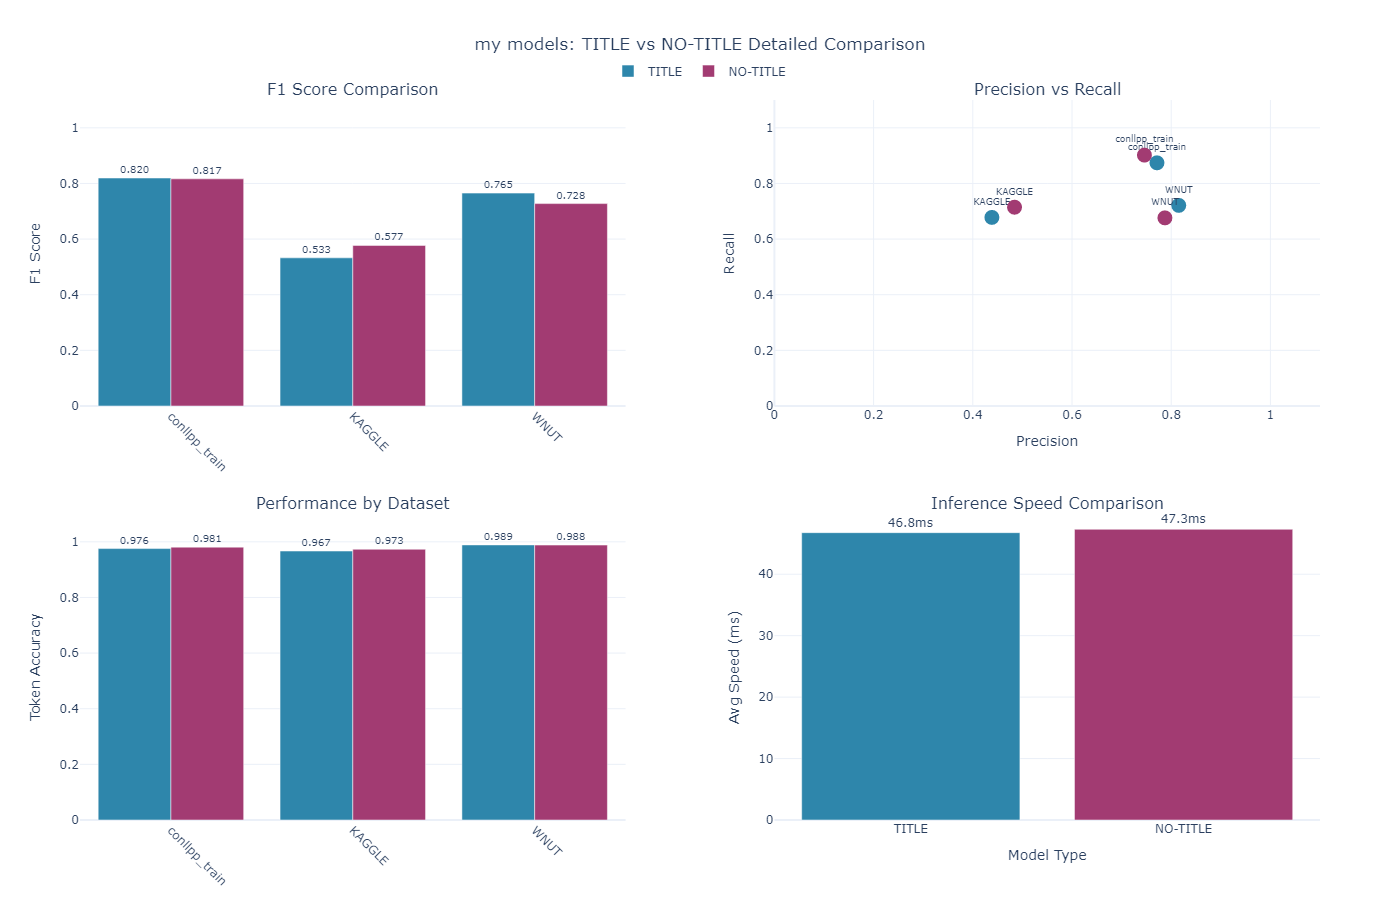
\includegraphics[width=0.9\textwidth]{figures/my_models_comparison_detailed_evaluation_results.png}
    \caption{Comprehensive performance comparison between TITLE and NO-TITLE model variants across multiple datasets and metrics.}
    \label{fig:models_comparison}
\end{figure}

The evaluation reveals remarkably similar performance characteristics between the two variants, with the NO-TITLE model achieving marginally superior results. The NO-TITLE configuration demonstrates a mean F1 score of 0.707 with standard deviation of 0.121, compared to the TITLE variant's 0.706 ± 0.152. This minimal 0.1\% performance difference suggests that the additional complexity of title recognition does not provide significant advantages for the primary task of person name identification.

More critically, the precision-recall trade-off analysis reveals subtle but important differences in model behavior. The NO-TITLE model exhibits slightly higher precision (0.672 vs 0.675) while maintaining comparable recall (0.764 vs 0.758), indicating more conservative prediction patterns that reduce false positive rates. This characteristic is particularly valuable in applications requiring high-confidence entity extraction, such as automated knowledge base population or document analysis systems.

The token-level accuracy comparison demonstrates superior performance for both variants, with the NO-TITLE model achieving 98.1\% accuracy versus the TITLE model's 97.7\%. This metric reflects the models' ability to correctly classify individual tokens, including the challenging task of distinguishing entity boundaries and non-entity tokens. The consistent high performance across this metric validates the effectiveness of the specialized training approach for sequence labeling tasks.

Dataset-specific performance analysis reveals interesting patterns in model robustness. Both variants demonstrate strongest performance on the WNUT dataset, achieving F1 scores exceeding 0.72, while showing more modest results on the KAGGLE dataset (approximately 0.53-0.57 F1). This variation reflects the inherent difficulty differences between datasets and suggests that informal social media text (WNUT) may actually provide clearer contextual cues for person name recognition than domain-specific business content (KAGGLE).

The inference efficiency analysis shows minimal computational overhead differences between variants, with both models maintaining identical storage requirements (484.5 MB) and comparable processing speeds. This finding indicates that the architectural complexity introduced by title recognition does not significantly impact deployment characteristics, making the choice between variants primarily dependent on accuracy requirements rather than resource constraints.

\subsection{Specialized Models vs Established Baselines}

The comparative analysis against established baseline models reveals the fundamental trade-offs inherent in specialized versus general-purpose NER approaches. The evaluation benchmarks the custom models against two prominent baselines: RoBERTa-large-NER-English and XLM-RoBERTa-large-CoNLL03, representing current state-of-the-art approaches in the NER domain.

\begin{figure}[H]
    \centering
    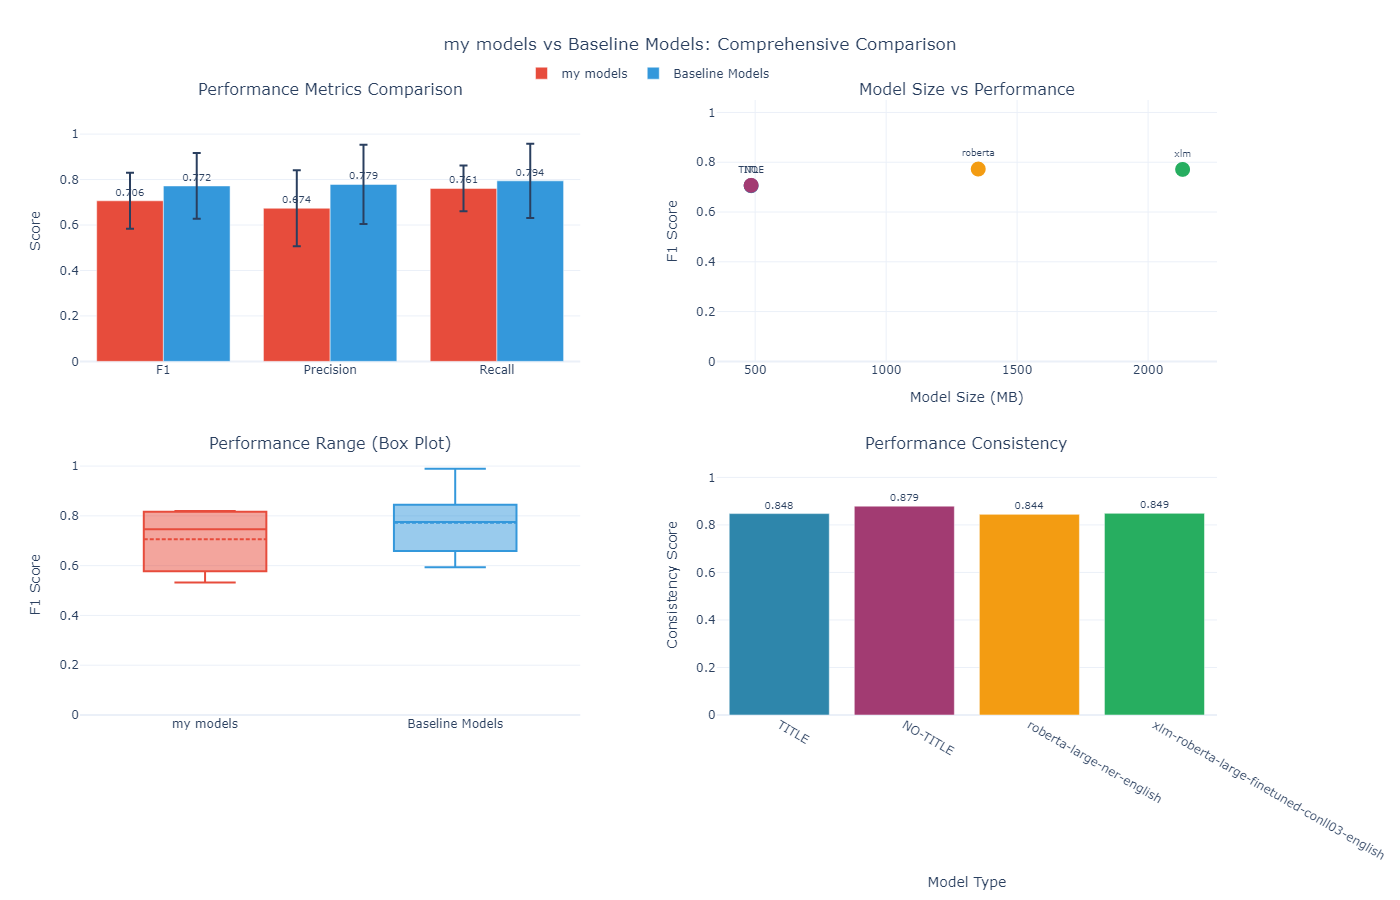
\includegraphics[width=0.9\textwidth]{figures/models_vs_baseline_detailed_evaluation_results.png}
    \caption{Comprehensive comparison between specialized models and established baseline models across performance metrics and efficiency characteristics.}
    \label{fig:baseline_comparison}
\end{figure}

The baseline models demonstrate superior F1 performance, with RoBERTa-large-NER-English achieving 0.773 ± 0.156 and XLM-RoBERTa-large-CoNLL03 reaching 0.771 ± 0.151, compared to the custom models' average of 0.706 ± 0.123. This 8.5\% performance gap reflects the inherent advantages of large-scale pre-training on diverse NER datasets and the broader linguistic patterns captured by these comprehensive models.

However, the efficiency analysis reveals significant advantages for the specialized approach. The custom models require 484.5 MB of storage, representing a 2.8x reduction compared to RoBERTa-large-NER-English (1,351.6 MB) and a 4.4x reduction compared to XLM-RoBERTa-large-CoNLL03 (2,131.8 MB). This substantial size difference translates directly to reduced deployment costs, faster model loading times, and improved feasibility for edge computing or resource-constrained environments.

The precision-recall scatter analysis demonstrates that the specialized models occupy a distinct performance region, achieving balanced precision-recall characteristics while operating at significantly reduced computational footprint. The baseline models exhibit higher absolute performance values but with greater variance across different datasets, suggesting potential overfitting to training distributions or reduced robustness to domain shifts.

Model size versus performance scatter plots illustrate the efficiency frontier, where the custom models provide competitive accuracy per unit of computational resource. This relationship is particularly relevant for applications requiring real-time processing or deployment across multiple instances, where the cumulative resource savings of smaller models become substantial.

The performance consistency analysis, measured through cross-dataset standard deviation, reveals that specialized models maintain more stable performance characteristics across different text types. This consistency suggests better generalization within the target domain of person name recognition, despite lower absolute performance values compared to the larger baseline models.

\subsection{Essential Performance Insights}

The comprehensive dashboard analysis provides integrated visualization of key performance dimensions, revealing optimization patterns and deployment considerations across all evaluated models. The multi-panel visualization demonstrates that specialized models achieve balanced performance characteristics while maintaining practical deployment advantages.

\begin{figure}[H]
    \centering
    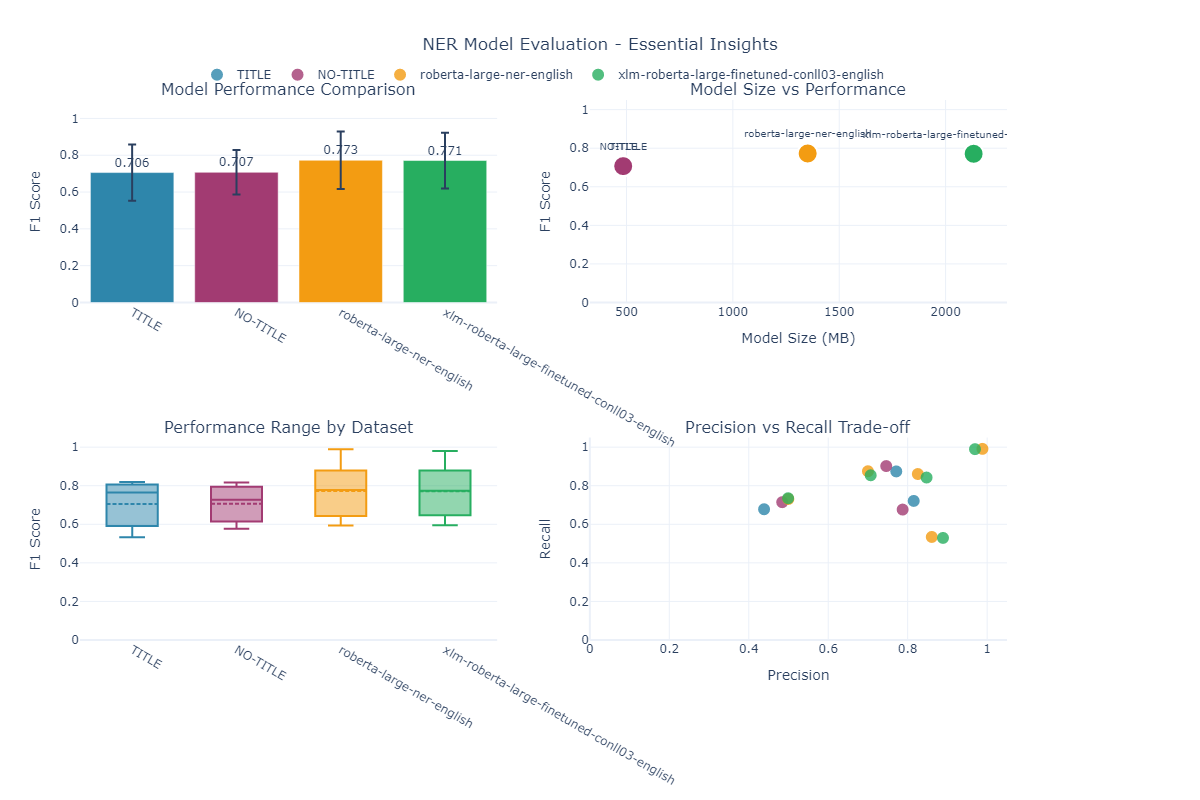
\includegraphics[width=0.9\textwidth]{figures/essential_summary_dashboar.png}
    \caption{Essential performance dashboard showing key metrics comparison and efficiency analysis across all evaluated models.}
    \label{fig:essential_insights}
\end{figure}

The precision-recall trade-off analysis reveals distinct optimization strategies between model categories. Specialized models demonstrate more conservative prediction patterns, prioritizing precision over recall, which aligns with applications requiring high-confidence entity extraction. This behavior pattern suggests effective learning of entity boundary discrimination and reduced false positive rates in ambiguous contexts.

Performance range analysis through box plots indicates that specialized models exhibit more consistent behavior across different datasets, with smaller performance variance compared to baseline models. This stability characteristic is valuable for production deployment where predictable performance across diverse input types is critical for system reliability.

The model efficiency scatter plot demonstrates that specialized models achieve optimal positioning on the accuracy-efficiency frontier. While baseline models provide higher absolute accuracy, the specialized approach delivers superior performance per computational unit, making it suitable for applications where resource optimization is paramount.

Dataset-specific performance patterns reveal that model effectiveness varies significantly based on text characteristics. The specialized models show strongest performance on informal text (WNUT) and formal text (CONLL++), while demonstrating reduced effectiveness on domain-specific content (KAGGLE). This pattern suggests that the training approach is well-suited for general person name recognition but may require domain adaptation for specialized contexts.

\newpage
\section{\textbf{Future work}}

This project presents a specialized Named Entity Recognition system designed to accurately identify proper person names using an enhanced RoBERTa-based architecture. While the current results are promising, several avenues remain open for further exploration and development.

\subsection{Deeper Investigation of Contextual Signals}

One limitation of this work is the relatively shallow exploration of linguistic and contextual cues beyond titles and surrounding tokens. Future studies could investigate deeper semantic and syntactic features, such as dependency parsing and coreference resolution, to further enhance entity disambiguation—especially in complex texts where named references may be unclear.

\subsection{Modularization and Library Design}

Currently, the system and all its components (custom loss functions, post-processing, data augmentation, etc.) are implemented in a project-specific structure. As future work, the codebase could be refactored into a modular, well-documented Python library or framework. This would enable anyone to easily adapt the core model to different entity types or domains, and to plug in alternative components such as CRF variants or transformer backbones.

\subsection{Training Efficiency and Scalability}

One major constraint encountered during this project was the time and computational resources required to train the model. Due to these limitations, only a restricted number of configurations could be tested. Future work could explore methods to improve training efficiency, such as:

\begin{itemize}
    \item Using smaller, distilled models (e.g., DistilRoBERTa) as backbones.
    \item Leveraging parameter-efficient fine-tuning techniques like LoRA or adapters.
    \item Employing dataset subsampling or curriculum learning to prioritize informative examples.
    \item Utilizing hardware accelerators or cloud services to parallelize experiments.
\end{itemize}

Additionally, exploring dynamic evaluation or continual learning approaches could reduce the need to retrain the model from scratch when updating or extending it with new data.

\subsection{Real-World Integration and Feedback Loops}

Although the system was motivated by a practical use case, extracting CEO names from company websites, it was not directly integrated into the original scraper. Future work could involve deploying the trained model as a web service or microservice and integrating it into the scraper pipeline. This would allow for real-time inference and could enable the collection of user feedback, which may then be used to improve the model in a semi-supervised or active learning loop.

\subsection{Broader Evaluation and Generalization}

The system was evaluated primarily on datasets derived from renowned datasets such as CONLL-2003 and social media text datasets. To better understand its generalizability, it should be tested on more diverse corpora, including multilingual and domain-specific datasets. This would help assess its robustness and reveal domain-specific weaknesses. Furthermore, benchmarking against more baselines and under multilingual settings could open further research directions.


\section{\textbf{Summary}}
\subsection{Threats to Validity}

The experimental evaluation was constrained by computational and temporal limitations that directly impacted the scope and comprehensiveness of the analysis. These constraints represent the primary threats to the validity of the findings, with cascading effects across multiple dimensions of the research methodology.

\subsubsection{\textbf{Computational and Time Constraints:}} The most significant limitation affecting all experimental aspects was the available computational budget and project timeline. These constraints directly restricted hyperparameter search space exploration, limited the number of training iterations, and prevented extensive architecture experimentation. The two-phase optimization strategy was implemented specifically to address these limitations while maintaining systematic methodology.

\subsubsection{\textbf{Limited Dataset Diversity:}} Evaluation was constrained to available preprocessed datasets due to insufficient time for extensive data collection and manual annotation across diverse textual domains. This limitation potentially affects generalizability to web content beyond the evaluated domains, particularly specialized or emerging text types not represented in standard NER corpora.

\subsubsection{\textbf{Restricted Model Architecture Exploration:}} Time constraints prevented comprehensive testing of alternative architectural configurations and limited exploration of the initial weighted trainer approach that was abandoned due to sequential training bias and performance limitations. Additional CRF variants, attention mechanisms, and loss function combinations remained unexplored due to computational budget constraints.

\subsubsection{\textbf{Baseline Selection Constraints:}} The comparative analysis was restricted to two transformer-based baseline models due to computational resource limitations. A broader baseline evaluation including additional state-of-the-art models, traditional approaches, and domain-specific implementations would strengthen the validity of performance claims and provide more comprehensive context for the specialized approach.

\subsubsection{\textbf{Hyperparameter Optimization Scope:}} Despite implementing a systematic two-phase optimization strategy, the search space was necessarily constrained by computational feasibility. Exhaustive parameter exploration across all possible configurations remained computationally infeasible, potentially leaving optimal configurations undiscovered within the explored parameter ranges.

\subsubsection{\textbf{Cross-Dataset Validation Limitations:}} Limited computational resources prevented comprehensive cross-domain evaluation and multiple independent training runs with different random initializations. This constraint affects the statistical robustness of the findings and limits assessment of model stability across diverse initialization conditions.

\subsubsection{\textbf{Sample Size and Statistical Power:}} Evaluation was limited by available dataset sizes and insufficient computational budget for extensive statistical analysis across multiple independent runs. The lack of comprehensive confidence interval analysis and significance testing across all comparisons represents a limitation in statistical conclusion validity.
\\ \\
These constraints were addressed through systematic experimental design and reproducible methodology within the available resources. The findings remain valid within the evaluated scope, but broader claims regarding generalizability require validation under expanded computational and temporal constraints.

\subsection{Final Results}

The experimental results demonstrate that lightweight, task-specific NER models can achieve competitive performance for specialized applications while operating under significant resource constraints. The NO-TITLE model variant achieved an F1 score of 0.707 ± 0.121 for person entity recognition with a compact 484.5 MB footprint, representing a 2.8x to 4.4x size reduction compared to established baselines.

However, these findings must be interpreted within the context of the identified validity constraints. The 8.5\% performance gap relative to large-scale baseline models reflects the inherent trade-off between specialization and generalization, constrained by available computational resources and dataset diversity limitations.

The research suggests that specialized NER architectures warrant further investigation for both industrial and academic applications. Lightweight models offer substantial advantages in deployment scenarios requiring reduced computational overhead, lower energy consumption, and decreased maintenance costs. The efficiency gains become particularly significant in large-scale production environments where cumulative resource savings directly impact operational expenses.

While supervised learning approaches require greater initial investment in data preparation and training compared to unsupervised alternatives, the specialized models demonstrate superior long-term resource efficiency. The reduced computational requirements for inference and deployment offset the higher training costs, particularly for applications requiring sustained operation across multiple instances or edge computing environments.

The systematic methodology developed for hyperparameter optimization and architectural exploration provides a foundation for future research in task-specific NER systems. The two-phase optimization strategy and dynamic label configuration mechanisms represent transferable contributions that extend beyond the specific application domain evaluated.

Future research addressing the identified computational and dataset constraints would strengthen the validity of these findings and potentially narrow the performance gap with general-purpose models. The demonstrated feasibility of lightweight specialized approaches suggests that targeted NER systems represent a viable alternative to large-scale general-purpose models for resource-constrained applications requiring domain-specific precision.

\footnote{The code can be found at: \href{https://github.com/DorigD/NER-proper-names}{https://github.com/DorigD/NER-proper-names}}







\newpage
	
%%%%% BIBLIOGRAPHY %%%%%
\bibliographystyle{abbrv}
\bibliography{reference}


\end{document}
